\documentclass{ximera}


\graphicspath{
  {./}
  {ximeraTutorial/}
  {basicPhilosophy/}
}

\newcommand{\mooculus}{\textsf{\textbf{MOOC}\textnormal{\textsf{ULUS}}}}


\usepackage{tkz-euclide}\usepackage{tikz}
\usepackage{tikz-cd}
\usetikzlibrary{arrows}
\tikzset{>=stealth,commutative diagrams/.cd,
  arrow style=tikz,diagrams={>=stealth}} %% cool arrow head
\tikzset{shorten <>/.style={ shorten >=#1, shorten <=#1 } } %% allows shorter vectors

\usetikzlibrary{backgrounds} %% for boxes around graphs
\usetikzlibrary{shapes,positioning}  %% Clouds and stars
\usetikzlibrary{matrix} %% for matrix
\usepgfplotslibrary{polar} %% for polar plots
\usepgfplotslibrary{fillbetween} %% to shade area between curves in TikZ
\usetkzobj{all}
\usepackage[makeroom]{cancel} %% for strike outs
%\usepackage{mathtools} %% for pretty underbrace % Breaks Ximera
%\usepackage{multicol}
\usepackage{pgffor} %% required for integral for loops



%% http://tex.stackexchange.com/questions/66490/drawing-a-tikz-arc-specifying-the-center
%% Draws beach ball
\tikzset{pics/carc/.style args={#1:#2:#3}{code={\draw[pic actions] (#1:#3) arc(#1:#2:#3);}}}



\usepackage{array}
\setlength{\extrarowheight}{+.1cm}
\newdimen\digitwidth
\settowidth\digitwidth{9}
\def\divrule#1#2{
\noalign{\moveright#1\digitwidth
\vbox{\hrule width#2\digitwidth}}}
























%%This is to help with formatting on future title pages.
\newenvironment{sectionOutcomes}{}{}



\title{Graphing}

\begin{document}
\begin{abstract}
polar coordinates
\end{abstract}
\maketitle

\section*{Polar Axes}



\begin{definition} \textbf{\textcolor{green!50!black}{Polar Coordinates}} \\
  An ordered pair consisting of a radius and an angle $(r,\theta)$
  can be plotted as

  \begin{image}[2in]
    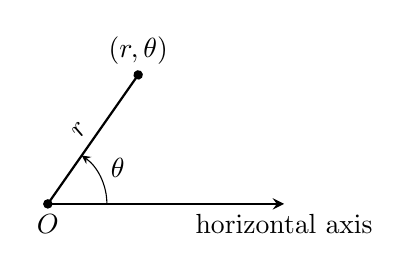
\begin{tikzpicture}
	\draw[thick,->] (0,0) node [below] {$O$} -- (3,0) node [below] {horizontal axis} ;
	\filldraw (0,0) circle (1.5pt);
	\filldraw [rotate=55] (2,0) circle (1.5pt);
	\draw [thick,rotate=55] (0,0)-- node [rotate=55,pos=.5,above] {$r$} (2,0) node [above] {$(r,\theta)$};
	\draw [->] (.75,0) arc(0:55:.75); 
	\draw [rotate=27.5] (1,0) node {$\theta$};
    \end{tikzpicture}
  \end{image}
  Coordinates of this type are called \textbf{polar coordinates}.
\end{definition}



If we view this point on a circle of radius $r$, then we can connect polar coordinates up to rectangular coordintes via our trigonometric functions.







\begin{image}[2in]
    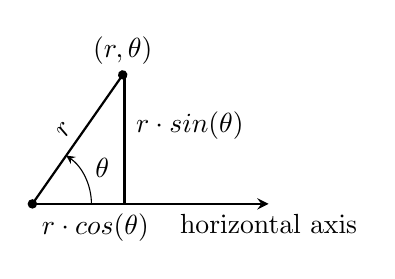
\begin{tikzpicture}
  \draw[thick,->] (0,0) -- (3,0) node [below] {horizontal axis} ;
  %\draw[thick,->] (0,0) node [below] {$O$} -- (3,0) node [below] {horizontal axis} ;
  \filldraw (0,0) circle (1.5pt);
  \filldraw [rotate=55] (2,0) circle (1.5pt);
  \draw [thick,rotate=55] (0,0)-- node [rotate=55,pos=.5,above] {$r$} (2,0) node [above] {$(r,\theta)$};
  \draw [->] (.75,0) arc(0:55:.75); 
  \draw [rotate=27.5] (1,0) node {$\theta$};




  \draw [thick] (1.17,0)--(1.17,1.6);
  \draw  (2,1) node {$r \cdot sin(\theta)$};
  \draw  (0.8,0) node [below] {$r \cdot cos(\theta)$};




    \end{tikzpicture}
  \end{image}

Bridge between polar and rectangular coordinates:
\begin{align*}
    x &= r\cdot \cos(\theta)\\
    y &= r\cdot \sin(\theta)
\end{align*}



















Polar coordinates are great for certain situations. However, there is
a price to pay. Every point in the plane has more than one
description in polar coordinates.





\begin{question}
  Which of the following represent the point, $(3,0)$, in
  $(x,y)$-coordinates?
  \begin{selectAll}
    \choice[correct]{$(3,0)$}
    \choice[correct]{$(3,2\pi)$}
    \choice{$(3,3\pi)$}
    \choice[correct]{$(3,-2\pi)$}
    \choice[correct]{$(3,4\pi)$}
  \end{selectAll}
  \begin{feedback}
    Any integer multiple of $2\pi$ will point towards the positive $x$-axis.
  \end{feedback}
\end{question}





\begin{question}
  Which of the following represent the origin, $(0,0)$, in
  $(x,y)$-coordinates?
  \begin{selectAll}
    \choice[correct]{$(0,0)$}
    \choice[correct]{$(0,\pi)$}
    \choice[correct]{$(0,\frac{\pi}{6})$}
    \choice[correct]{$(0,2\pi)$}
    \choice[correct]{$(0,-\pi)$}
  \end{selectAll}
  \begin{feedback}
    All of these represent the origin, since $(0,\theta)$ represents
    the origin for any angle $\theta$.
  \end{feedback}
\end{question}



What about a negative radius? How should we interpret a negative radius? 

$(-2,\pi)$ will mean to point in the $\pi$ direction and then move backwards $2$.  It describes the same point as $(2, 2\pi)$.









\begin{example}
Plot the following points described by the following polar coordinates:
\[
A =\left(1,\frac{\pi}{4}\right)\quad B=(1.5,\pi)\quad C = \left(2,-\frac{\pi}{3}\right)\quad D = \left(-1,\frac{\pi}{4}\right)
\]
\begin{explanation}
  It helps to use a ``polar grid'' to plot these points:
  \begin{image}
    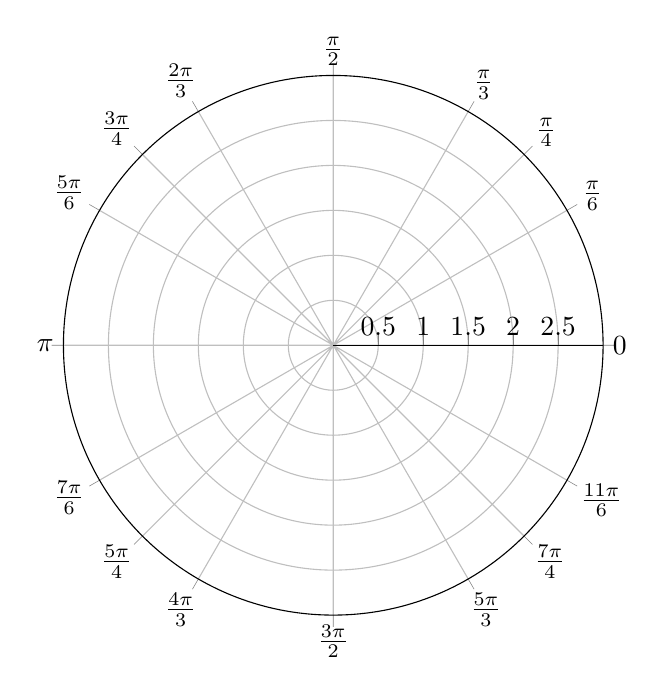
\begin{tikzpicture}
      \begin{polaraxis}[
          xmin=0,xmax=360, ymin=0,ymax=3,
          xtick={0,30,45,60,90,120,135,150,180,210,225,240,270,300,315,330,360},
          xticklabels={$0$,$\frac{\pi}{6}$,$\frac{\pi}{4}$,$\frac{\pi}{3}$,$\frac{\pi}{2}$,$\frac{2\pi}{3}$,$\frac{3\pi}{4}$,$\frac{5\pi}{6}$,$\pi$,$\frac{7\pi}{6}$,$\frac{5\pi}{4}$,$\frac{4\pi}{3}$,$\frac{3\pi}{2}$,$\frac{5\pi}{3}$,$\frac{7\pi}{4}$,$\frac{11\pi}{6}$,$2\pi$},
          ytick={.5,1,...,2.5},%yticklabels={},
        ]
        %\addplot+[draw=none, mark=none,penColor,domain=0:360,samples=100,smooth] {1};
      \end{polaraxis}
    \end{tikzpicture}
  \end{image}
  To place the point $A$, go out $1$ unit along the horizontal axis
  (putting you on the inner circle shown on the grid), then rotate
  \wordChoice{\choice{clockwise}\choice[correct]{counterclockwise}}
  $\frac{\pi}{4}$ radians (or $45^\circ$).
  
  To plot $B$, go out $1.5$ units along the horizontal axis and rotate
  $\pi$ radians ($180^\circ$).
  
  To plot $C$, go out 2 units along the initial ray then rotate
  \wordChoice{\choice[correct]{clockwise}\choice{counterclockwise}}
  $\frac{\pi}{3}$ radians, as the angle given is negative.

  To plot $D$, move along the initial ray ``$-1$'' units, in other
  words, ``back up'' $1$ unit, then rotate
  \wordChoice{\choice{clockwise}\choice[correct]{counterclockwise}} by
  $\frac{\pi}{4}$.
  \begin{hint}
    \begin{image}
      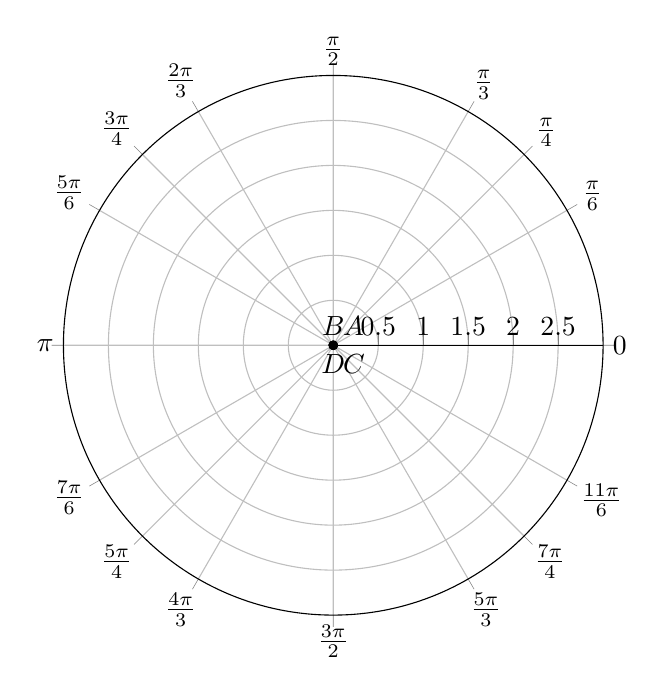
\begin{tikzpicture}
        \begin{polaraxis}[
            xmin=0,xmax=360, ymin=0,ymax=3,
            xtick={0,30,45,60,90,120,135,150,180,210,225,240,270,300,315,330,360},
            xticklabels={$0$,$\frac{\pi}{6}$,$\frac{\pi}{4}$,$\frac{\pi}{3}$,$\frac{\pi}{2}$,$\frac{2\pi}{3}$,$\frac{3\pi}{4}$,$\frac{5\pi}{6}$,$\pi$,$\frac{7\pi}{6}$,$\frac{5\pi}{4}$,$\frac{4\pi}{3}$,$\frac{3\pi}{2}$,$\frac{5\pi}{3}$,$\frac{7\pi}{4}$,$\frac{11\pi}{6}$,$2\pi$},
            ytick={.5,1,...,2.5},%yticklabels={},
          ]
          \filldraw [rotate=45] (100,0) circle (1.5pt) node [above right] {$A$};
          \filldraw [rotate=180] (150,0) circle (1.5pt) node [above] {$B$};
          \filldraw [rotate=-60] (200,0) circle (1.5pt) node [below right] {$C$};
          \filldraw [rotate=45] (-100,0) circle (1.5pt) node [below] {$D$};
        \end{polaraxis}
      \end{tikzpicture}
    \end{image}
  \end{hint}
\end{explanation}
\end{example}


















It is useful to recognize both the rectangular (Cartesian)
coordinates of a point in the plane and the polar coordinates.

\begin{theorem}  \textbf{\textcolor{green!50!black}{Cartesian - Polar Bridge}} \\

Given a point $P=(r,\theta)$ in polar coordinates, rectangular
coordinates are given by
\[
x=r\cos(\theta)\qquad y=r\sin(\theta).
\]
Given a point $Q=(x,y)$ in rectangular coordinates, polar coordinates
are given by
\[
r^2=x^2+y^2\qquad \tan(\theta) = \frac{y}{x}.
\]
\end{theorem}





\begin{question}
  Let $P=\left( 2,\frac{2\pi}{3} \right)$ be a point in polar coordinates. Describe $P$ in
  rectangular coordinates.
    \[
    P = \left( \answer{1}, \answer{\sqrt{3}} \right)
    \]
\end{question}

  \begin{question}
  Let $Q=(-1,\frac{5\pi}{4})$ be a point in polar coordinates. Describe $Q$ in
  rectangular coordinates.
    \[
    Q = \left( \answer{1\sqrt{2}}, \answer{1\sqrt{2}} \right)
    \]
\end{question}


\begin{question}
  Let $P=(1,2)$ be a point in rectangular coordinates. Describe $P$ in
  polar coordinates.
    \[
    P = \left( \answer{\sqrt{5}}, \arctan(2) \right)
    \]
\end{question}


  \begin{question}
  Let $Q=(-1,1)$ be a point in rectangular coordinates. Describe $Q$ in
  polar coordinates.

    \[
    Q = \left( \answer{-\sqrt{2}}, \arctan(-1) \right)
    \]
    \begin{hint}
      We'll tell you the angle, you think about the radius.
    \end{hint}
\end{question}



















\section*{Polar Graphs}

Let's talk about how to plot polar functions in the two coordinate systems.  \\


We can plot points on rectangular axes thinking $y = r(\theta)$. 





\begin{example}
  Sketch the polar function $r=1+\cos(\theta)$ on $[0,2\pi]$ with rectangular coordinates.  \\


  $\theta$ will be measured along the horzontal axis and $r$ will be measured along the vertical axis.

    \begin{image}%% 45
      \begin{tikzpicture}
  \begin{axis}[
            domain=0:2*pi,
            xmin=-.3,xmax=6.32,ymin=-.3,ymax=2.3,
            axis lines =middle, xlabel=$\theta$, ylabel=$y$,
            every axis y label/.style={at=(current axis.above origin),anchor=south},
            every axis x label/.style={at=(current axis.right of origin),anchor=west},
            xtick={0,.785,...,6.28},
            xticklabels={$0$,$\frac{\pi}{4}$,$\frac{\pi}{2}$,$\frac{3\pi}{4}$,$\pi$,$\frac{5\pi}{4}$,$\frac{3\pi}{2}$,$\frac{7\pi}{4}$,$2\pi$},
            ytick={0,1,2},
          ]
          %\addplot [dashed, smooth,] {1+cos(deg(x)};
          \addplot [very thick, penColor, smooth,domain=0:6.28] {1+cos(deg(x))};
        \end{axis}
      \end{tikzpicture}
      \end{image}
\end{example}


Another graphing option is a polar coordinate system.  Instead of measuring $\theta$ horizontally, we measure it as a counterclockwise turn.  Instead of measuring $r$ vertically, we measure it away from the origin in the direction $\theta$.

In the Cartesian graph, $r$ begins at a height of $2$ and then moves down as $\theta$ moves to the right.

In the Polar graph, we turn counterclockwise to an angle of $\theta$ and then move in that direction to a radial measurement of $r$. So, we turn to $0$ radians with a distance of $2$.  As $\theta$ grows, we turn counterclockwise and the radial measurement shortens,

\begin{image}
\begin{tikzpicture}
          \begin{polaraxis}[
              xtick={0,45,...,360},
              xticklabels={$0$,$\frac{\pi}{4}$,$\frac{\pi}{2}$,$\frac{3\pi}{4}$,$\pi$,$\frac{5\pi}{4}$,$\frac{3\pi}{2}$,$\frac{7\pi}{4}$,$2\pi$},
              ytick={.5,1,...,2},
            ]
            \addplot+[very thick, mark=none,penColor,domain=0:45,samples=100,smooth] {1+cos(x)};
          \end{polaraxis}
\end{tikzpicture}
\end{image}



Then we continue turning counterclockwise and moving the radial measurement in and out until you get around the whole circle.


\begin{example}
  Sketch the polar function $r=1+\cos(\theta)$ on $[0,2\pi]$.
  \begin{explanation} 

Begin at $0$ radians and work your way counterclockwise easy angles moving $r$ closer to the origin or further way.

    
    \begin{image}%% 45
      \begin{tikzpicture}
	\begin{axis}[
            domain=0:2*pi,
            xmin=-.3,xmax=6.32,ymin=-.3,ymax=2.3,
            axis lines =middle, xlabel=$x$, ylabel=$y$,
            every axis y label/.style={at=(current axis.above origin),anchor=south},
            every axis x label/.style={at=(current axis.right of origin),anchor=west},
            xtick={0,.785,...,6.28},
            xticklabels={$0$,$\frac{\pi}{4}$,$\frac{\pi}{2}$,$\frac{3\pi}{4}$,$\pi$,$\frac{5\pi}{4}$,$\frac{3\pi}{2}$,$\frac{7\pi}{4}$,$2\pi$},
            ytick={0,1,2},
          ]
          \addplot [dashed, smooth,] {1+cos(deg(x)};
	  \addplot [very thick, penColor, smooth,domain=0:.785] {1+cos(deg(x)};
        \end{axis}
      \end{tikzpicture}
      \qquad
       \begin{tikzpicture}
          \begin{polaraxis}[
              xtick={0,45,...,360},
              xticklabels={$0$,$\frac{\pi}{4}$,$\frac{\pi}{2}$,$\frac{3\pi}{4}$,$\pi$,$\frac{5\pi}{4}$,$\frac{3\pi}{2}$,$\frac{7\pi}{4}$,$2\pi$},
              ytick={.5,1,...,2},
            ]
            \addplot+[very thick, mark=none,penColor,domain=0:45,samples=100,smooth] {1+cos(x)};
          \end{polaraxis}
         \end{tikzpicture}
    \end{image}

    
    \begin{image}%% 90
      \begin{tikzpicture}
	\begin{axis}[
            domain=0:2*pi,
            xmin=-.3,xmax=6.32,ymin=-.3,ymax=2.3,
            axis lines =middle, xlabel=$x$, ylabel=$y$,
            every axis y label/.style={at=(current axis.above origin),anchor=south},
            every axis x label/.style={at=(current axis.right of origin),anchor=west},
            xtick={0,.785,...,6.28},
            xticklabels={$0$,$\frac{\pi}{4}$,$\frac{\pi}{2}$,$\frac{3\pi}{4}$,$\pi$,$\frac{5\pi}{4}$,$\frac{3\pi}{2}$,$\frac{7\pi}{4}$,$2\pi$},
            ytick={0,1,2},
          ]
          \addplot [dashed, smooth,] {1+cos(deg(x)};
	  \addplot [very thick, penColor, smooth,domain=0:1.57] {1+cos(deg(x))};
        \end{axis}
      \end{tikzpicture}
      \qquad
      \begin{tikzpicture}
          \begin{polaraxis}[
              xtick={0,45,...,360},
              xticklabels={$0$,$\frac{\pi}{4}$,$\frac{\pi}{2}$,$\frac{3\pi}{4}$,$\pi$,$\frac{5\pi}{4}$,$\frac{3\pi}{2}$,$\frac{7\pi}{4}$,$2\pi$},
              ytick={.5,1,...,2},
            ]
            \addplot+[very thick, mark=none,penColor,domain=0:90,samples=100,smooth] {1+cos(x)};
          \end{polaraxis}
         \end{tikzpicture}
    \end{image}
    
    
    \begin{image}%% 135
      \begin{tikzpicture}
	\begin{axis}[
            domain=0:2*pi,
            xmin=-.3,xmax=6.32,ymin=-.3,ymax=2.3,
              axis lines =middle, xlabel=$x$, ylabel=$y$,
              every axis y label/.style={at=(current axis.above origin),anchor=south},
              every axis x label/.style={at=(current axis.right of origin),anchor=west},
              xtick={0,.785,...,6.28},
              xticklabels={$0$,$\frac{\pi}{4}$,$\frac{\pi}{2}$,$\frac{3\pi}{4}$,$\pi$,$\frac{5\pi}{4}$,$\frac{3\pi}{2}$,$\frac{7\pi}{4}$,$2\pi$},
              ytick={0,1,2},
            ]
            \addplot [dashed, smooth,] {1+cos(deg(x)};
	    \addplot [very thick, penColor, smooth,domain=0:2.355] {1+cos(deg(x))};
          \end{axis}
        \end{tikzpicture}
        \qquad
        \begin{tikzpicture}
          \begin{polaraxis}[
              xtick={0,45,...,360},
              xticklabels={$0$,$\frac{\pi}{4}$,$\frac{\pi}{2}$,$\frac{3\pi}{4}$,$\pi$,$\frac{5\pi}{4}$,$\frac{3\pi}{2}$,$\frac{7\pi}{4}$,$2\pi$},
              ytick={.5,1,...,2},
            ]
            \addplot+[very thick, mark=none,penColor,domain=0:135,samples=100,smooth] {1+cos(x)};
          \end{polaraxis}
         \end{tikzpicture}
      \end{image}

    
       \begin{image}%% 180
         \begin{tikzpicture}
	   \begin{axis}[
               domain=0:2*pi,
               xmin=-.3,xmax=6.32,ymin=-.3,ymax=2.3,
               axis lines =middle, xlabel=$x$, ylabel=$y$,
               every axis y label/.style={at=(current axis.above origin),anchor=south},
              every axis x label/.style={at=(current axis.right of origin),anchor=west},
              xtick={0,.785,...,6.28},
              xticklabels={$0$,$\frac{\pi}{4}$,$\frac{\pi}{2}$,$\frac{3\pi}{4}$,$\pi$,$\frac{5\pi}{4}$,$\frac{3\pi}{2}$,$\frac{7\pi}{4}$,$2\pi$},
              ytick={0,1,2},
             ]
            \addplot [dashed, smooth,] {1+cos(deg(x)};
	    \addplot [very thick, penColor, smooth,domain=0:3.14] {1+cos(deg(x))};
           \end{axis}
        \end{tikzpicture}
        \qquad
         \begin{tikzpicture}
          \begin{polaraxis}[
              xtick={0,45,...,360},
              xticklabels={$0$,$\frac{\pi}{4}$,$\frac{\pi}{2}$,$\frac{3\pi}{4}$,$\pi$,$\frac{5\pi}{4}$,$\frac{3\pi}{2}$,$\frac{7\pi}{4}$,$2\pi$},
              ytick={.5,1,...,2},
            ]
            \addplot+[very thick, mark=none,penColor,domain=0:180,samples=100,smooth] {1+cos(x)};
          \end{polaraxis}
         \end{tikzpicture}
      \end{image}

       
       \begin{image}%% 225
         \begin{tikzpicture}
	   \begin{axis}[
               domain=0:2*pi,
               xmin=-.3,xmax=6.32,ymin=-.3,ymax=2.3,
               axis lines =middle, xlabel=$x$, ylabel=$y$,
               every axis y label/.style={at=(current axis.above origin),anchor=south},
              every axis x label/.style={at=(current axis.right of origin),anchor=west},
              xtick={0,.785,...,6.28},
              xticklabels={$0$,$\frac{\pi}{4}$,$\frac{\pi}{2}$,$\frac{3\pi}{4}$,$\pi$,$\frac{5\pi}{4}$,$\frac{3\pi}{2}$,$\frac{7\pi}{4}$,$2\pi$},
              ytick={0,1,2},
             ]
            \addplot [dashed, smooth,] {1+cos(deg(x)};
	    \addplot [very thick, penColor, smooth,domain=0:3.93] {1+cos(deg(x))};
           \end{axis}
        \end{tikzpicture}
        \qquad
        \begin{tikzpicture}
          \begin{polaraxis}[
              xtick={0,45,...,360},
              xticklabels={$0$,$\frac{\pi}{4}$,$\frac{\pi}{2}$,$\frac{3\pi}{4}$,$\pi$,$\frac{5\pi}{4}$,$\frac{3\pi}{2}$,$\frac{7\pi}{4}$,$2\pi$},
              ytick={.5,1,...,2},
            ]
            \addplot+[very thick, mark=none,penColor,domain=0:225,samples=100,smooth] {1+cos(x)};
          \end{polaraxis}
         \end{tikzpicture}
       \end{image}

       
       \begin{image}%% 270
         \begin{tikzpicture}
	   \begin{axis}[
               domain=0:2*pi,
               xmin=-.3,xmax=6.32,ymin=-.3,ymax=2.3,
               axis lines =middle, xlabel=$x$, ylabel=$y$,
               every axis y label/.style={at=(current axis.above origin),anchor=south},
              every axis x label/.style={at=(current axis.right of origin),anchor=west},
              xtick={0,.785,...,6.28},
              xticklabels={$0$,$\frac{\pi}{4}$,$\frac{\pi}{2}$,$\frac{3\pi}{4}$,$\pi$,$\frac{5\pi}{4}$,$\frac{3\pi}{2}$,$\frac{7\pi}{4}$,$2\pi$},
              ytick={0,1,2},
             ]
            \addplot [dashed, smooth,] {1+cos(deg(x)};
	    \addplot [very thick, penColor, smooth,domain=0:4.71] {1+cos(deg(x))};
           \end{axis}
        \end{tikzpicture}
        \qquad
        \begin{tikzpicture}
          \begin{polaraxis}[
              xtick={0,45,...,360},
              xticklabels={$0$,$\frac{\pi}{4}$,$\frac{\pi}{2}$,$\frac{3\pi}{4}$,$\pi$,$\frac{5\pi}{4}$,$\frac{3\pi}{2}$,$\frac{7\pi}{4}$,$2\pi$},
              ytick={.5,1,...,2},
            ]
            \addplot+[very thick, mark=none,penColor,domain=0:270,samples=100,smooth] {1+cos(x)};
          \end{polaraxis}
         \end{tikzpicture}
       \end{image}

       
       \begin{image}%% 315
         \begin{tikzpicture}
	   \begin{axis}[
               domain=0:2*pi,
               xmin=-.3,xmax=6.32,ymin=-.3,ymax=2.3,
               axis lines =middle, xlabel=$x$, ylabel=$y$,
               every axis y label/.style={at=(current axis.above origin),anchor=south},
              every axis x label/.style={at=(current axis.right of origin),anchor=west},
              xtick={0,.785,...,6.28},
              xticklabels={$0$,$\frac{\pi}{4}$,$\frac{\pi}{2}$,$\frac{3\pi}{4}$,$\pi$,$\frac{5\pi}{4}$,$\frac{3\pi}{2}$,$\frac{7\pi}{4}$,$2\pi$},
              ytick={0,1,2},
             ]
            \addplot [dashed, smooth,] {1+cos(deg(x)};
	    \addplot [very thick, penColor, smooth,domain=0:5.5] {1+cos(deg(x))};
           \end{axis}
        \end{tikzpicture}
        \qquad
        \begin{tikzpicture}
          \begin{polaraxis}[
              xtick={0,45,...,360},
              xticklabels={$0$,$\frac{\pi}{4}$,$\frac{\pi}{2}$,$\frac{3\pi}{4}$,$\pi$,$\frac{5\pi}{4}$,$\frac{3\pi}{2}$,$\frac{7\pi}{4}$,$2\pi$},
              ytick={.5,1,...,2},
            ]
            \addplot+[very thick, mark=none,penColor,domain=0:315,samples=100,smooth] {1+cos(x)};
          \end{polaraxis}
         \end{tikzpicture}
       \end{image}

       
       \begin{image}%% 360
         \begin{tikzpicture}
	   \begin{axis}[
               domain=0:2*pi,
               xmin=-.3,xmax=6.32,ymin=-.3,ymax=2.3,
               axis lines =middle, xlabel=$x$, ylabel=$y$,
               every axis y label/.style={at=(current axis.above origin),anchor=south},
              every axis x label/.style={at=(current axis.right of origin),anchor=west},
              xtick={0,.785,...,6.28},
              xticklabels={$0$,$\frac{\pi}{4}$,$\frac{\pi}{2}$,$\frac{3\pi}{4}$,$\pi$,$\frac{5\pi}{4}$,$\frac{3\pi}{2}$,$\frac{7\pi}{4}$,$2\pi$},
              ytick={0,1,2},
             ]
            \addplot [dashed, smooth,] {1+cos(deg(x)};
	    \addplot [very thick, penColor, smooth,domain=0:6.28] {1+cos(deg(x))};
           \end{axis}
        \end{tikzpicture}
        \qquad
        \begin{tikzpicture}
          \begin{polaraxis}[
              xtick={0,45,...,360},
              xticklabels={$0$,$\frac{\pi}{4}$,$\frac{\pi}{2}$,$\frac{3\pi}{4}$,$\pi$,$\frac{5\pi}{4}$,$\frac{3\pi}{2}$,$\frac{7\pi}{4}$,$2\pi$},
              ytick={.5,1,...,2},
            ]
            \addplot+[very thick, mark=none,penColor,domain=0:360,samples=100,smooth] {1+cos(x)};
          \end{polaraxis}
         \end{tikzpicture}
       \end{image}
  \end{explanation}
\end{example}











\begin{example}
  Sketch the polar function $r=\cos(2 \theta)$ on $[0,2\pi]$.
  \begin{explanation}
   Begin at $0^{\circ}$, move counterclockwise to easy angles, plot radius.  Then sketch in the graph..
    \begin{image}%% 45
      \begin{tikzpicture}
	\begin{axis}[
            domain=0:2*pi,
            xmin=-.3,xmax=6.32,ymin=-1.3,ymax=1.3,
            axis lines =middle, xlabel=$x$, ylabel=$y$,
            every axis y label/.style={at=(current axis.above origin),anchor=south},
            every axis x label/.style={at=(current axis.right of origin),anchor=west},
            xtick={0,.785,...,6.28},
            xticklabels={$0$,$\frac{\pi}{4}$,$\frac{\pi}{2}$,$\frac{3\pi}{4}$,$\pi$,$\frac{5\pi}{4}$,$\frac{3\pi}{2}$,$\frac{7\pi}{4}$,$2\pi$},
            ytick={0,1,2},
          ]
          \addplot [dashed, smooth,] {cos(2*deg(x))};
	  \addplot [very thick, penColor, smooth,domain=0:.785] {cos(2*deg(x)};
        \end{axis}
      \end{tikzpicture}
      \qquad
      \begin{tikzpicture}
          \begin{polaraxis}[
              xtick={0,45,...,360},
              xticklabels={$0$,$\frac{\pi}{4}$,$\frac{\pi}{2}$,$\frac{3\pi}{4}$,$\pi$,$\frac{5\pi}{4}$,$\frac{3\pi}{2}$,$\frac{7\pi}{4}$,$2\pi$},
              ytick={.25,.5,...,1},
            ]
            \addplot+[very thick, mark=none,penColor,domain=0:45,samples=100,smooth] {cos(2*x)};
          \end{polaraxis}
         \end{tikzpicture}
    \end{image}

    
    \begin{image}%% 90
      \begin{tikzpicture}
	\begin{axis}[
            domain=0:2*pi,
            xmin=-.3,xmax=6.32,ymin=-1.3,ymax=1.3,
            axis lines =middle, xlabel=$x$, ylabel=$y$,
            every axis y label/.style={at=(current axis.above origin),anchor=south},
            every axis x label/.style={at=(current axis.right of origin),anchor=west},
            xtick={0,.785,...,6.28},
            xticklabels={$0$,$\frac{\pi}{4}$,$\frac{\pi}{2}$,$\frac{3\pi}{4}$,$\pi$,$\frac{5\pi}{4}$,$\frac{3\pi}{2}$,$\frac{7\pi}{4}$,$2\pi$},
            ytick={0,1,2},
          ]
          \addplot [dashed, smooth,] {cos(2*deg(x))};
	  \addplot [very thick, penColor, smooth,domain=0:1.57] {cos(2*deg(x))};
        \end{axis}
      \end{tikzpicture}
      \qquad
      \begin{tikzpicture}
          \begin{polaraxis}[
              xtick={0,45,...,360},
              xticklabels={$0$,$\frac{\pi}{4}$,$\frac{\pi}{2}$,$\frac{3\pi}{4}$,$\pi$,$\frac{5\pi}{4}$,$\frac{3\pi}{2}$,$\frac{7\pi}{4}$,$2\pi$},
              ytick={.25,.5,...,1},
            ]
            \addplot+[very thick, mark=none,penColor,domain=0:90,samples=100,smooth] {cos(2*x)};
          \end{polaraxis}
         \end{tikzpicture}
    \end{image}
    
    
    \begin{image}%% 135
      \begin{tikzpicture}
	\begin{axis}[
            domain=0:2*pi,
            xmin=-.3,xmax=6.32,ymin=-1.3,ymax=1.3,
              axis lines =middle, xlabel=$x$, ylabel=$y$,
              every axis y label/.style={at=(current axis.above origin),anchor=south},
              every axis x label/.style={at=(current axis.right of origin),anchor=west},
              xtick={0,.785,...,6.28},
              xticklabels={$0$,$\frac{\pi}{4}$,$\frac{\pi}{2}$,$\frac{3\pi}{4}$,$\pi$,$\frac{5\pi}{4}$,$\frac{3\pi}{2}$,$\frac{7\pi}{4}$,$2\pi$},
              ytick={0,1,2},
            ]
            \addplot [dashed, smooth,] {cos(2*deg(x))};
	    \addplot [very thick, penColor, smooth,domain=0:2.355] {cos(2*deg(x))};
          \end{axis}
        \end{tikzpicture}
        \qquad
        \begin{tikzpicture}
          \begin{polaraxis}[
              xtick={0,45,...,360},
              xticklabels={$0$,$\frac{\pi}{4}$,$\frac{\pi}{2}$,$\frac{3\pi}{4}$,$\pi$,$\frac{5\pi}{4}$,$\frac{3\pi}{2}$,$\frac{7\pi}{4}$,$2\pi$},
              ytick={.25,.5,...,1},
            ]
            \addplot+[very thick, mark=none,penColor,domain=0:135,samples=100,smooth] {cos(2*x)};
          \end{polaraxis}
         \end{tikzpicture}
      \end{image}

    
       \begin{image}%% 180
         \begin{tikzpicture}
	   \begin{axis}[
               domain=0:2*pi,
               xmin=-.3,xmax=6.32,ymin=-1.3,ymax=1.3,
               axis lines =middle, xlabel=$x$, ylabel=$y$,
               every axis y label/.style={at=(current axis.above origin),anchor=south},
              every axis x label/.style={at=(current axis.right of origin),anchor=west},
              xtick={0,.785,...,6.28},
              xticklabels={$0$,$\frac{\pi}{4}$,$\frac{\pi}{2}$,$\frac{3\pi}{4}$,$\pi$,$\frac{5\pi}{4}$,$\frac{3\pi}{2}$,$\frac{7\pi}{4}$,$2\pi$},
              ytick={0,1,2},
             ]
            \addplot [dashed, smooth,] {cos(2*deg(x))};
	    \addplot [very thick, penColor, smooth,domain=0:3.14] {cos(2*deg(x))};
           \end{axis}
        \end{tikzpicture}
        \qquad
        \begin{tikzpicture}
          \begin{polaraxis}[
              xtick={0,45,...,360},
              xticklabels={$0$,$\frac{\pi}{4}$,$\frac{\pi}{2}$,$\frac{3\pi}{4}$,$\pi$,$\frac{5\pi}{4}$,$\frac{3\pi}{2}$,$\frac{7\pi}{4}$,$2\pi$},
              ytick={.25,.5,...,1},
            ]
            \addplot+[very thick, mark=none,penColor,domain=0:180,samples=100,smooth] {cos(2*x)};
          \end{polaraxis}
         \end{tikzpicture}
      \end{image}

       
       \begin{image}%% 225
         \begin{tikzpicture}
	   \begin{axis}[
               domain=0:2*pi,
               xmin=-.3,xmax=6.32,ymin=-1.3,ymax=1.3,
               axis lines =middle, xlabel=$x$, ylabel=$y$,
               every axis y label/.style={at=(current axis.above origin),anchor=south},
              every axis x label/.style={at=(current axis.right of origin),anchor=west},
              xtick={0,.785,...,6.28},
              xticklabels={$0$,$\frac{\pi}{4}$,$\frac{\pi}{2}$,$\frac{3\pi}{4}$,$\pi$,$\frac{5\pi}{4}$,$\frac{3\pi}{2}$,$\frac{7\pi}{4}$,$2\pi$},
              ytick={0,1,2},
             ]
            \addplot [dashed, smooth,] {cos(2*deg(x))};
	    \addplot [very thick, penColor, smooth,domain=0:3.93] {cos(2*deg(x))};
           \end{axis}
        \end{tikzpicture}
        \qquad
        \begin{tikzpicture}
          \begin{polaraxis}[
              xtick={0,45,...,360},
              xticklabels={$0$,$\frac{\pi}{4}$,$\frac{\pi}{2}$,$\frac{3\pi}{4}$,$\pi$,$\frac{5\pi}{4}$,$\frac{3\pi}{2}$,$\frac{7\pi}{4}$,$2\pi$},
              ytick={.25,.5,...,1},
            ]
            \addplot+[very thick, mark=none,penColor,domain=0:225,samples=100,smooth] {cos(2*x)};
          \end{polaraxis}
         \end{tikzpicture}
       \end{image}

       
       \begin{image}%% 270
         \begin{tikzpicture}
	   \begin{axis}[
               domain=0:2*pi,
               xmin=-.3,xmax=6.32,ymin=-1.3,ymax=1.3,
               axis lines =middle, xlabel=$x$, ylabel=$y$,
               every axis y label/.style={at=(current axis.above origin),anchor=south},
              every axis x label/.style={at=(current axis.right of origin),anchor=west},
              xtick={0,.785,...,6.28},
              xticklabels={$0$,$\frac{\pi}{4}$,$\frac{\pi}{2}$,$\frac{3\pi}{4}$,$\pi$,$\frac{5\pi}{4}$,$\frac{3\pi}{2}$,$\frac{7\pi}{4}$,$2\pi$},
              ytick={0,1,2},
             ]
            \addplot [dashed, smooth,] {cos(2*deg(x))};
	    \addplot [very thick, penColor, smooth,domain=0:4.71] {cos(2*deg(x))};
           \end{axis}
        \end{tikzpicture}
        \qquad
        \begin{tikzpicture}
          \begin{polaraxis}[
              xtick={0,45,...,360},
              xticklabels={$0$,$\frac{\pi}{4}$,$\frac{\pi}{2}$,$\frac{3\pi}{4}$,$\pi$,$\frac{5\pi}{4}$,$\frac{3\pi}{2}$,$\frac{7\pi}{4}$,$2\pi$},
              ytick={.25,.5,...,1},
            ]
            \addplot+[very thick, mark=none,penColor,domain=0:270,samples=100,smooth] {cos(2*x)};
          \end{polaraxis}
         \end{tikzpicture}		
       \end{image}

       
       \begin{image}%% 315
         \begin{tikzpicture}
	   \begin{axis}[
               domain=0:2*pi,
               xmin=-.3,xmax=6.32,ymin=-1.3,ymax=1.3,
               axis lines =middle, xlabel=$x$, ylabel=$y$,
               every axis y label/.style={at=(current axis.above origin),anchor=south},
              every axis x label/.style={at=(current axis.right of origin),anchor=west},
              xtick={0,.785,...,6.28},
              xticklabels={$0$,$\frac{\pi}{4}$,$\frac{\pi}{2}$,$\frac{3\pi}{4}$,$\pi$,$\frac{5\pi}{4}$,$\frac{3\pi}{2}$,$\frac{7\pi}{4}$,$2\pi$},
              ytick={0,1,2},
             ]
            \addplot [dashed, smooth,] {cos(2*deg(x))};
	    \addplot [very thick, penColor, smooth,domain=0:5.5] {cos(2*deg(x))};
           \end{axis}
        \end{tikzpicture}
        \qquad
        \begin{tikzpicture}
          \begin{polaraxis}[
              xtick={0,45,...,360},
              xticklabels={$0$,$\frac{\pi}{4}$,$\frac{\pi}{2}$,$\frac{3\pi}{4}$,$\pi$,$\frac{5\pi}{4}$,$\frac{3\pi}{2}$,$\frac{7\pi}{4}$,$2\pi$},
              ytick={.25,.5,...,1},
            ]
            \addplot+[very thick, mark=none,penColor,domain=0:315,samples=100,smooth] {cos(2*x)};
          \end{polaraxis}
         \end{tikzpicture}
       \end{image}

       
       \begin{image}%% 360
         \begin{tikzpicture}
	   \begin{axis}[
               domain=0:2*pi,
               xmin=-.3,xmax=6.32,ymin=-1.3,ymax=1.3,
               axis lines =middle, xlabel=$x$, ylabel=$y$,
               every axis y label/.style={at=(current axis.above origin),anchor=south},
              every axis x label/.style={at=(current axis.right of origin),anchor=west},
              xtick={0,.785,...,6.28},
              xticklabels={$0$,$\frac{\pi}{4}$,$\frac{\pi}{2}$,$\frac{3\pi}{4}$,$\pi$,$\frac{5\pi}{4}$,$\frac{3\pi}{2}$,$\frac{7\pi}{4}$,$2\pi$},
              ytick={0,1,2},
             ]
            \addplot [dashed, smooth,] {cos(2*deg(x))};
	    \addplot [very thick, penColor, smooth,domain=0:6.28] {cos(2*deg(x))};
           \end{axis}
        \end{tikzpicture}
        \qquad
        \begin{tikzpicture}
          \begin{polaraxis}[
              xtick={0,45,...,360},
              xticklabels={$0$,$\frac{\pi}{4}$,$\frac{\pi}{2}$,$\frac{3\pi}{4}$,$\pi$,$\frac{5\pi}{4}$,$\frac{3\pi}{2}$,$\frac{7\pi}{4}$,$2\pi$},
              ytick={.25,.5,...,1},
            ]
            \addplot+[very thick, mark=none,penColor,domain=0:360,samples=100,smooth] {cos(2*x)};
          \end{polaraxis}
         \end{tikzpicture}
       \end{image}
  \end{explanation}
\end{example}



















\section*{Converting to and from Polar Coordinates}


It is sometimes desirable to refer to a graph via a polar equation,
and other times by a rectangular equation.  Therefore it is necessary
to be able to convert between polar and rectangular coordinates.  Here
is the basic idea:

Given a function $y=f(x)$ in rectangular coordinates, polar coordinates
are given by setting
\[
x=r\cos(\theta)\qquad y=r\sin(\theta).
\]
and solving for $r$.

Given a function $r(\theta)$ in polar coordinates, rectangular
coordinates harder to find. The basic idea is to ``find'' $r\cdot
\cos(\theta)$ and $r\cdot \sin(\theta)$ and write:
\[
r\cos(\theta) = x\qquad r\sin(\theta) = y.
\]
Sometimes it is useful to remember that:
\[
r^2=x^2+y^2\qquad \tan \theta = \frac yx.
\]


\begin{example}
  Convert $y=x^2$ from rectangular coordinates to polar coordinates.
  \begin{explanation}
    Replace $y$ with $r\sin(\theta)$ and replace $x$ with $r\cos(\theta)$, giving:
      \begin{align*}
	y &=x^2\\
	r\sin(\theta) &= \answer[given]{r^2\cos^2(\theta)}\\
	\answer[given]{\frac{\sin(\theta)}{\cos^2(\theta)}}  &= r.
      \end{align*}
      We have found that $r=\frac{\sin(\theta)}{\cos^2(\theta)}$. 

      One connected piece of the domain of this polar function is $\left( \frac{-\pi}{2}, \frac{\pi}{2} \right)$. This will trace out the entire graph.




      Since cosine is $0$ at $\frac{-\pi}{2}$ and $\frac{-\pi}{2}$, and it is in the denominator of our expression for $r$, we see that $r$ is unbounded at the ends of our domain interval.  This is how the ends of the parabola achieved.





  \end{explanation}







\begin{center}
\desmos{fmqxmo1pbs}{400}{300}
\end{center}



\end{example}






\begin{warning}
      When $\theta$ is inside $\left( \frac{-\pi}{2}, 0 \right)$, then our direction is into the fourth quadrant.  However, $\sin(\theta) < 0$ in the fourth quadrant, which means $r < 0$.  This means we are plotting points in the second quadrant, which is where the parabola is.


      When $\theta$ is inside $\left( 0, \frac{\pi}{2} \right)$, then our direction is into the first quadrant.   $\sin(\theta) > 0$ in the first quadrant, which means $r > 0$.  This means we are plotting points in the first quadrant, which is where the parabola is.


      $\theta = 0$ needs some thought.  When $\theta = 0$, then $\sin(\theta) = 0$ and $r = 0$.  That gives us the Cartesian point $(0,0)$, which is the bottom point on the parabola.  But, if $r =$ here, then how did we divide both sides of our equation above by $r$?

      Just as algebraic thinking, there was a factor of $r$ on both and we divided both sides by $r$.  This is simply symbolic manipulation according to the symbols and operations.  When we thinking funationally or analytically, then we need to be thinking about possible values.

      In this case, we might just talk about $\theta = 0$ separately, by itself, and then let the algebra descibe the rest of the points.  The $r$ will never equal $0$ and our division is ok.
\end{warning}







\begin{idea}  



Rather than dividing both sides by $r$, we might bring everything to one side of the equation with $0$ on the other side.



\[ r \sin(\theta) - r^2 \cos(\theta) = 0   \]


Factor, 

\[ r (\sin(\theta) - r \cos(\theta)) = 0   \]



Either $r = 0$ or $(\sin(\theta) - r \cos(\theta)) = 0$.

We could think about $r=0$ and then we could think about $(\sin(\theta) - r \cos(\theta)) = 0$ with $r \ne 0$.


Function analysis requires us to keep track of all of the loose ends that algebraic symbolic manipulation just doesn;t care about.



\end{idea}












\begin{example}
  Convert $xy = 1$ from rectangular coordinates to polar coordinates.
  \begin{explanation}
    We again replace $x$ and $y$ using the standard identities and
    work to solve for $r$:
    \begin{align*}
	xy &= 1 \\
	\answer[given]{r\cos(\theta)\cdot r\sin(\theta)} & = 1\\
	r^2 & = \frac{1}{\cos(\theta)\sin(\theta)}\\
	r & = \frac{1}{\sqrt{\cos(\theta)\sin(\theta)}}\\
    \end{align*}
    This function is valid only when the product of
    $\cos(\theta) \sin(\theta)$ is positive. This occurs in the first and
    third quadrants, meaning the domain of this polar function is
    $(0,\tfrac{\pi}{2})$ with $(\pi,\tfrac{3\pi}{2})$.
      
    We can rewrite the original rectangular equation $xy=1$ as
    $y=\frac{1}{x}$. Note it only exists in the first and third quadrants.
  \end{explanation}
\end{example}





\begin{example}
   Convert $r=\frac{2}{\sin(\theta)-\cos(\theta)}$ from polar coordinates
   to rectangular coordinates.
   \begin{explanation}
     There is no set way to convert from polar to rectangular; in
     general, we look to form the products $r\cos(\theta)$ and
     $r\sin(\theta)$, and then replace these with $x$ and $y$,
     respectively. We start in this situation by multiplying both sides
     by $\sin(\theta)-\cos(\theta)$:
     \begin{align*}
       r &= \frac{2}{\sin(\theta)-\cos(\theta)} \\
       r(\sin(\theta)-\cos(\theta)) &= 2\\
       \answer[given]{r\sin(\theta)}-r\cos(\theta) &= 2. \qquad \text{Now replace with $y$ and $x$:}\\
       y-x &= 2\\
	  y &= x+2.
     \end{align*}
     The original polar equation, $r=\frac{2}{(\sin(\theta)-\cos(\theta))}$ does
     not easily reveal that its graph is simply a line. However, our
     conversion shows that it is.
   \end{explanation}
\end{example}

\begin{example}
   Convert $r =2\cos(\theta)$ from polar coordinates to rectangular
   coordinates.        	
   \begin{explanation}
     By multiplying both sides by $r$, we obtain both an $r^2$ term
     and an $r\cos(\theta)$ term, which we replace with $x^2+y^2$ and
     $x$, respectively.
     \begin{align*}
       r &=2\cos(\theta) \\
       r^2 &= 2r\cos(\theta) \\
       \answer[given]{x^2+y^2} &= \answer[given]{2x}. 
     \end{align*}
     We recognize this as a circle. By completing the square we can
     find its radius and center.
     \begin{align*}
       x^2-2x+y^2 &= 0 \\
       \answer[given]{(x-1)^2 + y^2} &=1.
     \end{align*}
     The circle is centered at $(1,0)$ and has radius $1$.
   \end{explanation}
 \end{example}
















\begin{center}
\textbf{\textcolor{green!50!black}{ooooo-=-=-=-ooOoo-=-=-=-ooooo}} \\

more examples can be found by following this link\\ \link[More Examples of Polar Graphs]{https://ximera.osu.edu/csccmathematics/precalculus2/precalculus2/polarGraphing/examples/exampleList}

\end{center}





\end{document}
